\documentclass[12pt]{article}
\usepackage{geometry}
 \geometry{
 a4paper,
 total={210mm,297mm},
 left=32mm,
 right=32mm,
 top=30mm,
 bottom=30mm,
 }
\usepackage[utf8]{inputenc}
\usepackage[ngerman]{babel}
\usepackage{fancyhdr}
\usepackage{graphicx}
\usepackage{tikz}
\pagestyle{plain}
\usepackage{hyperref}




\author{Konstantin Wirz/Matrikelnummer : 8124396}
\title{Grundpraktikum Programmierung(01584)/WS 2014}


\begin{document}



\maketitle

\tableofcontents

\section{Einleitung}

Im Rahmen vom 'Grundpraktikum Programmierung' wurde ein Werkzeug (Editor) zum Editieren und Simulieren von Petrinetzen entwickelt.

\emph{YAPNE} (Yet Another Petri Net Editor) wurde auf dem Mac OS X 10.10.1 entwickelt und getestet, Java Version "1.7.0\_60-ea".


\section{Grundidee, Konzepte und Designentscheidungen}
Anwendung ist in 2 Schichten aufgeteilt: Model und Präsentation. Model-Schicht repräsentiert Elemente aus der Petri Netz Domäne und Präsentation-Schicht ist grafische Darstellung dieser Elemente. Dadurch ist saubere Trennung zwischen Kernfunktionalität des Netzes und der grafischen Darstellung erreicht. Anwendung besteht aus 5 Packages, die hier erklärt werden. \\

\subsection{Package \emph{de.kwirz.yapne.model}}

Model-Schicht ist im \emph{de.kwirz.yapne.model} Package untergebracht und ist folgendermaßen aufgebaut.\\
\includegraphics[width=\linewidth]{model}

Alle Klassen in diesem Package implementieren \emph{PNMLable} Interface, das heißt sie können ihren aktuellen Status als \textbf{PNML} zurückgeben.

\emph{PetriNetElement} ist eine abstrakte Basisklasse für alle Elemente des Petri Netzes, also Stellen, Transitionen und Kanten, alle diese Elemente besitzen eine Id. Eine weitere abstrakte Basisklasse ist \emph{PetriNetNode}, die einen Knoten, also Stelle oder Transition repräsentiert. \emph{PetriNetNode} kann einen Namen haben, sowie Eingangs- und Ausgangskanten und eine Position, die durch eingebettete \emph{Position} Klasse repräsentiert ist. Zwei Kinderklassen der \emph{PetriNetNode} Klasse sind \emph{PetriNetPlace} und \emph{PetriNetTransition}, die weitere spezifische Details für Stellen und Transitionen implementieren. \emph{PetriNetPlace} repräsentiert eine Stelle und implementiert Markierung-Eigenschaft. \emph{PetriNetTransition} repräsentiert eine Transition, liefert mit \emph{isEnabled()} Methode ob sie aktiviert ist und kann mittels \emph{occur()} geschaltet werden. Ein weiteres Kind der \emph{PetriNetElement} Klasse ist \emph{PetriNetArc} Klasse, die eine Kante repräsentiert. \emph{PetriNetArc} kann Eingangs- und Ausgangsknoten haben.

\emph{PetriNet} repräsentiert das gesamte Petri Netz und bietet die Möglichkeit an, Stellen, Transitionen und Kanten zu verwalten. Da diese Elemente eine gemeinsame Basisklasse \emph{PetriNeElement} haben werden sie dem Netz mit Hilfe der Methode \emph{addElement(PetriNetElement element)} hinzugefügt. Sonstige Operationen auf Elementen Menge, wie Existenz überprüfen, Element entfernen, Element holen, erfolgen über Id, was für alle Petri Netz Elemente eindeutig sein sollte. Beim Entfernen von Transitionen und Stellen werden Eingangs- sowie Ausgangskanten dieser Elemente mit entfernt. Mit Hilfe der Methode \emph{getIds()} können Kennungen aller Elemente im Petri Netz geholt werden, Methode \emph{clear()} entfernt alle Elemente aus dem Petri Netz. Da \emph{PetriNet} \emph{PNMLable} Interface implementiert, kann mit Hilfe von \emph{toPNML()} Methode der aktuelle Status des gesamtes Netzes geholt werden und z.B. auf sekundären Speicher für weitere Bearbeitung gespeichert. 

\subsection{Package \emph{de.kwirz.yapne.presentation}}

Jetzt kommen wir zur Präsentation-Schicht, die sich im \emph{de.kwirz.yapne.presentation} Package befindet. \\
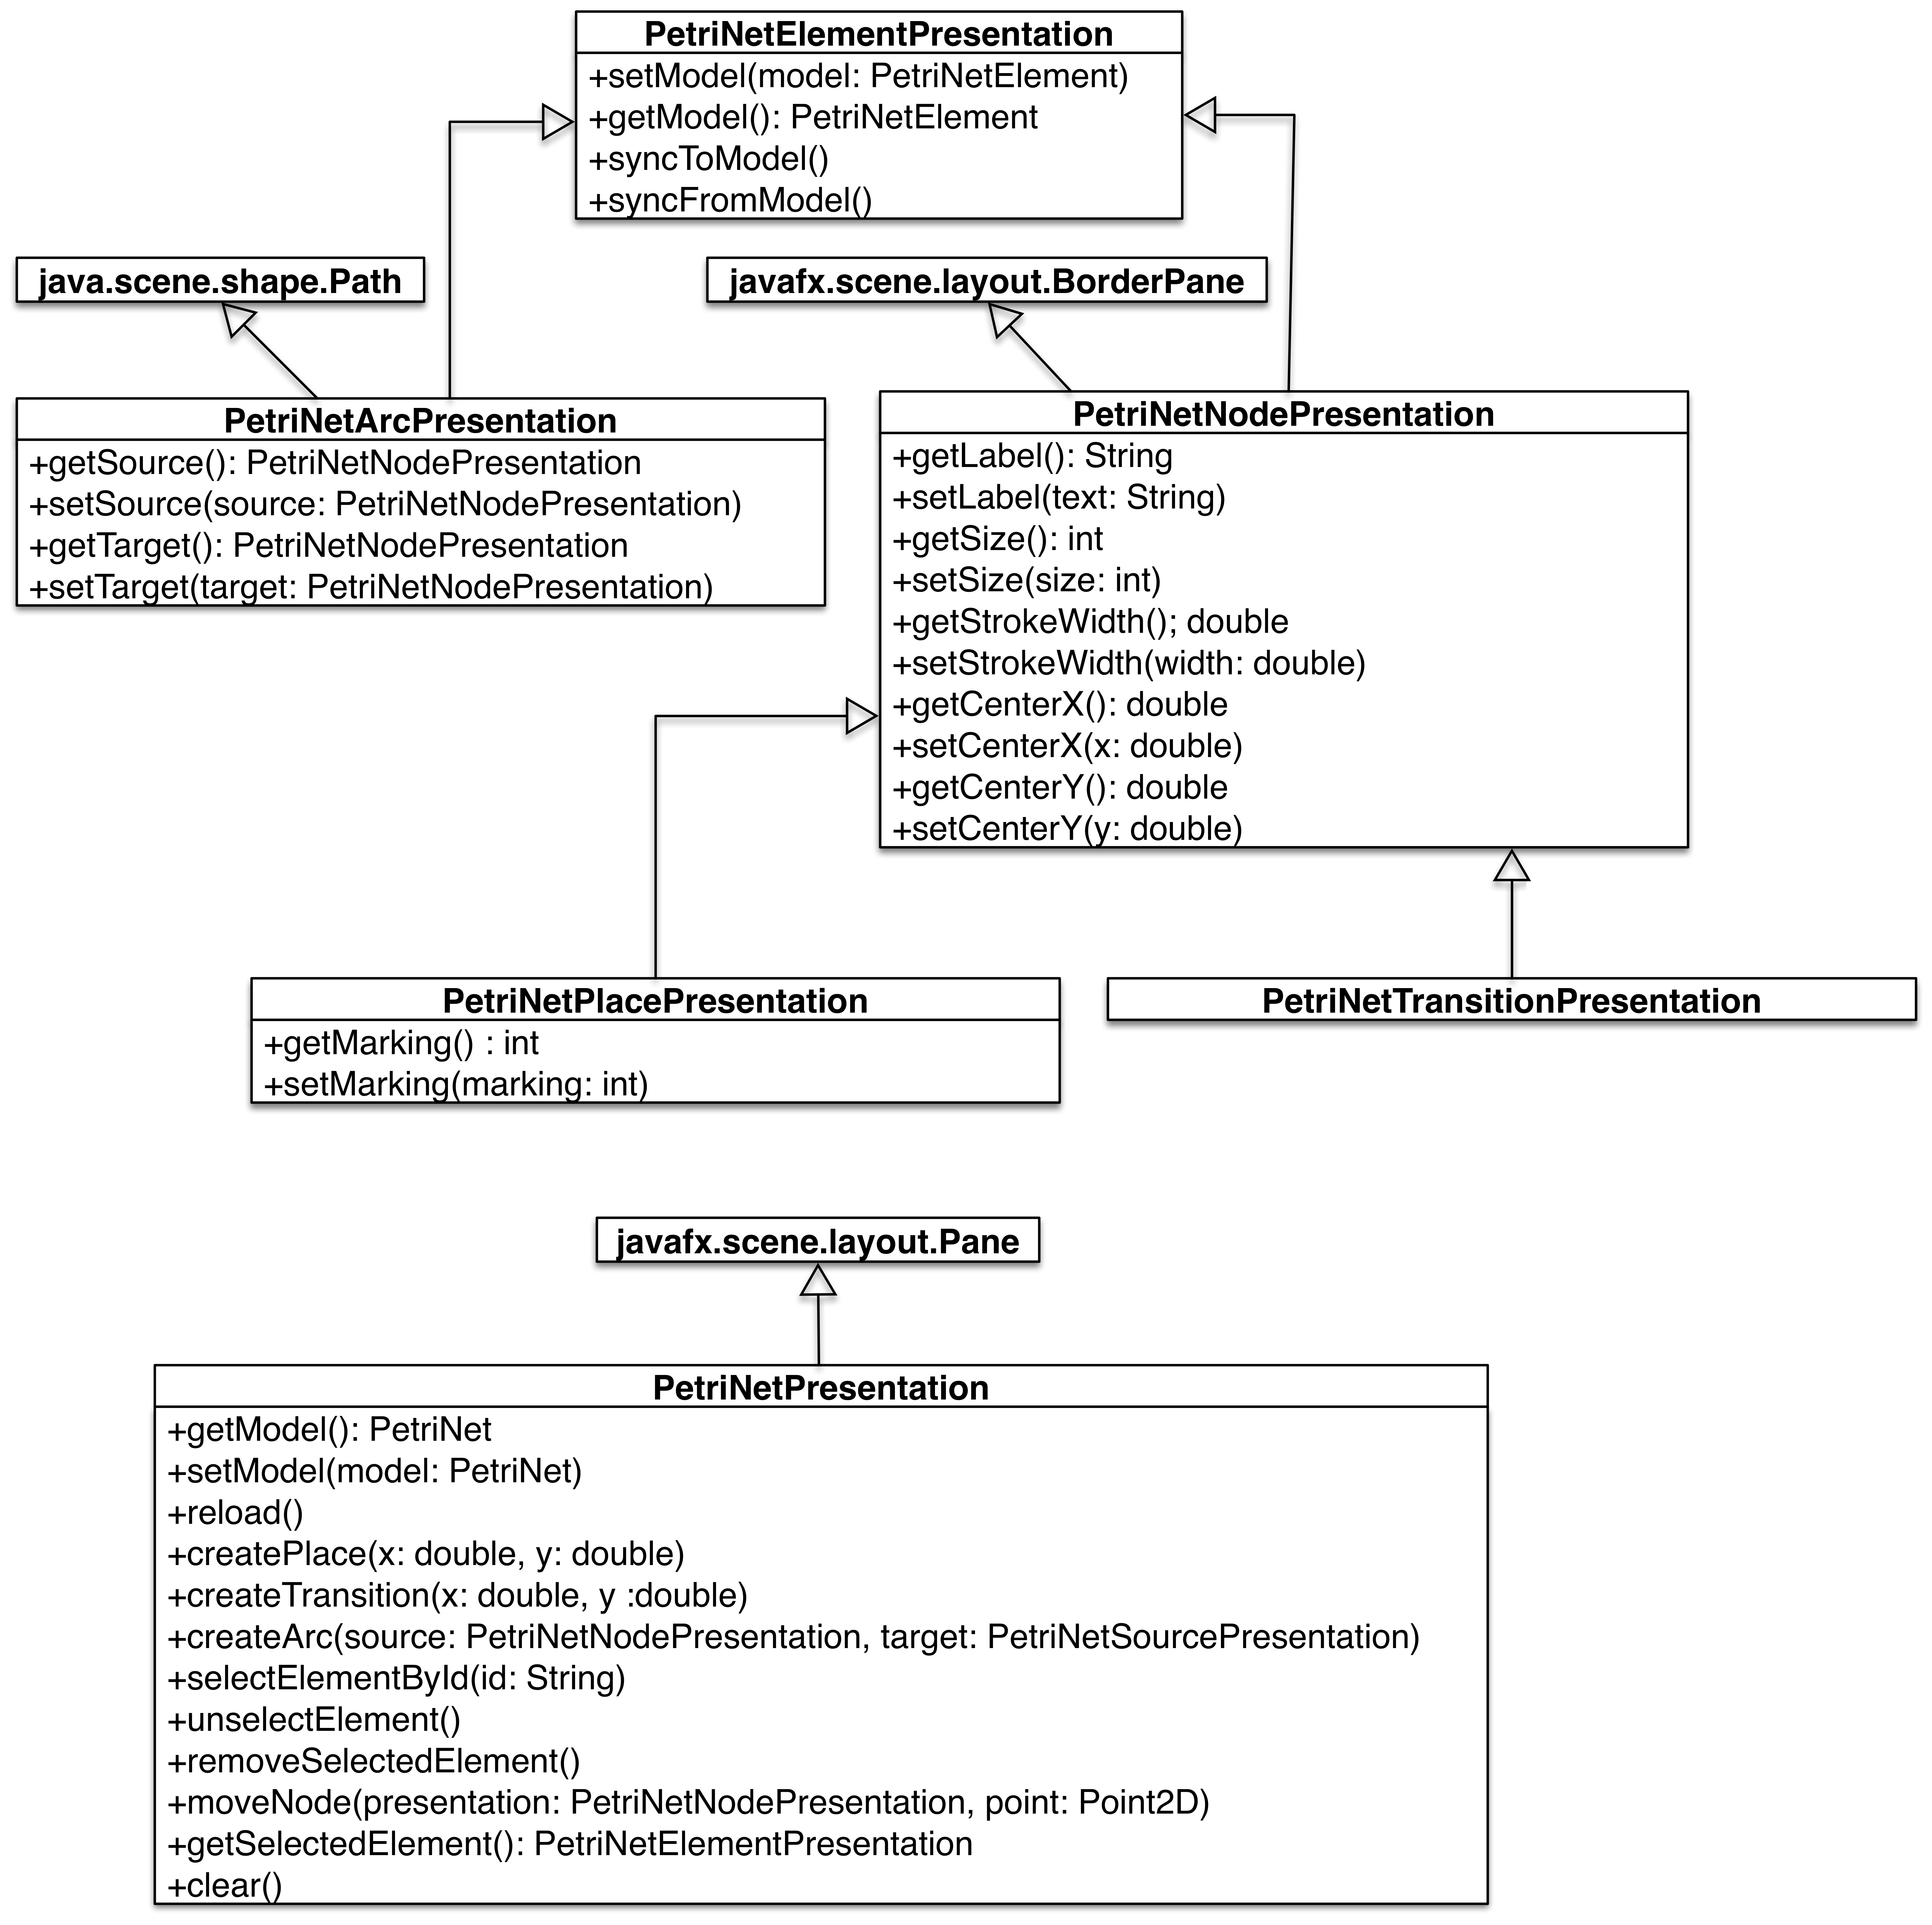
\includegraphics[width=\linewidth]{presentation}

Diese Klassen sind grafische Darstellungen der aus dem \emph{model} Package stammenden Modele. Element-Präsentationen implementieren Interface
\emph{PetriNetElementPresentation}, das folgende Methoden deklariert:
\begin{itemize}
\item{setModel() - setzt den Model}
\item{getModel() - gibt den Model zurück}
\item{syncToModel() - schreibt Daten in den Model}
\item{syncFromModel() - liest Daten aus dem Model}
\end{itemize}
Sollte sich die Präsentation ändern, dann werden die Daten in den Model geschrieben via \emph{syncToModel}. Hat sich der Model geändert, werden die Daten aus dem Model gelesen via \emph{syncFromModel}. Als Alternative könnte man jede Änderung die in den konkreten Methoden gemacht wurde, in den Model schreiben lassen, das wäre aber nicht mehr kontrollierbar für Benutzer dieser Klassen.

\emph{PetriNetNodePresentation} ist eine grafische Darstellung eines Knoten (Stelle, Transition), Klasse erbt von \emph{javafx.scene.layout.BorderPane}, die \textbf{Top} Position von \emph{BorderPane} wird für Anzeige der Knotennamen beansprucht, die \textbf{Center} Position wird von Kinderklassen gesetzt. \emph{PetriNetPlacePresentation} setzt als \textbf{Center} einen Kreis mit der Markierung in der Mitte, \emph{PetriNetTransitionPresentation} ein Quadrat.

\emph{PetriNetArcPresentation} ist eine grafische Darstellung einer Kante, nachdem Source und Target Eigenschaften mit \emph{setSource(PetriNetNodePresentation node)} und \emph{setTarget(PetriNetNodePresentation node)} gesetzt sind, zeichnet die Klasse eine Gerade von Mittelpunkt des Quellknoten bis Mittelpunkt des Zielknotens mit einem Pfeil am Ende. Die Gerade startet und endet an den Außenkanten. Werden Ziel- oder Quellknoten bewegt, aktualisiert sich auch die Kante.

\emph{PetriNetPresentation} ist eine grafische Darstellung eines Petri Netzes. Nach dem der Model gesetzt ist, werden für jedes Element des Models korrespondierende Präsentation erstellt und dargestellt. Außerdem können Elemente aus- und abgewählt werden, entfernt sowie der aktuelle Model kann neu gezeichnet werden.

\subsection{Package \emph{de.kwirz.yapne.app}}

Der Einstiegspunkt der Anwendung, sowie ihre Steuerung befinden sich in \emph{de.\\kwirz.yapne.app} Package. Die Klasse \emph{App} 
lädt Benutzerschnittstelle aus einer \textbf{FXML} Datei, initialisiert den Controller \emph{AppController}, der auch weitere Steuerung
übernimmt.

\emph{AppController} reagiert auf unterschiedliche Benutzeraktionen, Methoden den Controller sind als Handler in \textbf{FXML} Datei gesetzt, die beim aktivieren bestimmter Elemente ausgeführt werden. So werden z.B. solche Aktionen wie \textbf{Neue Datei}, \textbf{Datei Speichern}, \textbf{Einstellungen}, \textbf{Programm beenden} usw. vom Controller behandelt.


Weitere Klassen in diesem Package sind \emph{Dialogs}, \emph{SettingsDialog}, \emph{MessageBox}. \emph{Dialogs} und \emph{MessageBox} sind einfache Implementierungen der fehlenden in JavaFX 2.2 Dialogen und Message Boxen. Klasse \emph{SettingsDialog} ist der Einstellungsdialog dieser Anwendung.

\subsection{Package \emph{de.kwirz.yapne.io}}

Einzige Klasse in diesem Package ist \emph{PnmlParser}. Die ist für das Parsen von \textbf{PNML} Dateien zuständig, mittels der Methode \emph{parse(String input)}, die eine Instanz von \emph{PetriNet} zurückgibt.

\subsection{Package \emph{de.kwirz.yapne.utils}}

Dieses Package enthält unterschiedliche Hilfsklassen: \emph{Utils}, \emph{BuilderValue} und \emph{Settings}. Klasse \emph{BuilderValue} wird in Builder-Entwurfsmuster Implementierungen benutzt. Klasse \emph{Settings} ist für das Lesen und Schreiben von Einstellungen zuständig, dafür wird eine Datei im Home-Verzeichnis angelegt. Klasse \emph{Utils} enthält verschiedene statische Hilfsfunktionen.


\section{Bedienhandbuch}


\end{document}
